\section{Tests}
In this section, we present two sets of test cases to validate the results we obtained with the formulations we derived. The first case is the biaxial tension test which is used to calibrate material constants. For isotropic materials, the analytical solution is easy to find. The second case is the expansion of a vessel, which is a very representative application in the field of biomechanics.  

\subsection{Biaxial Tension Test}
A long bar loaded equally in two directions with fixed tractions is considered. The section is a $1$ $m^2$ square. Define the stretch $\lambda$ as the ratio between the deformed length to the original length, then for isotropic incompressible material, the stress is easy to find.
\begin{equation}
S_{11} = S_{22} = 2(1 - {\lambda}^{-6})(\frac{\partial\Psi_{iso}}{\partial\bar{I}_1} + {\lambda}^2\frac{\partial\Psi_{iso}}{\partial\bar{I}_2}), \quad S_{33} = 0
\end{equation}
where $S_{11}$, $S_{22}$, $S_{33}$ are the diagonal components of the PK2 stress, all the off-diagonal components are $0$.

Denote the nonzero component of PK2 stress as $S$. For Mooney-Rivlin model, plug in Equation \ref{iso1}, we have

\begin{equation}
S = (1 - {\lambda}^{-6})(\mu_1 + \mu_2{\lambda}^2)
\end{equation}
and therefore the nominal stress $P$ is
\begin{equation}
P = \lambda S =  (\lambda - {\lambda}^{-5})(\mu_1 + \mu_2{\lambda}^2)
\end{equation}
Neglecting the $\mu_2$ terms we have the nominal stresse for Neo-Hookean model
\begin{equation}
P = \lambda S =  \mu_1(\lambda - {\lambda}^{-5})
\end{equation}
Similarly, for Yeoh model
\begin{equation}
P = \lambda S = 2(\lambda - {\lambda}^{-5})[c_1 + 2c_2(2{\lambda}^2 + {\lambda}^{-4} - 3) + 3c_3(2{\lambda}^2 + {\lambda}^{-4} - 3)^2]
\end{equation}

The material constants used in these models are curve-fitted from the standard ASTM412 tensile test results of the same material. See Shashikant. In Neo-Hookean model, $\mu_1 = 0.6548$ MPa; in Mooney-Rivlin model, $\mu_1 = 0.595522$ MPa, $\mu_2 = -0.0508009$ MPa; in Yeoh model, $c_1 = 0.358756$ MPa, $c_2 = - 0.0508009$ MPa, $c_3 = 0.0142132$ MPa. The Poisson's ratios for all the models are over $\nu = 0.49999$, closed enough to incompressibility.

Figure \ref{fig:biaxial1} shows the results of the theoretical calculation and numerical computation. Perfect agreement is achieved. As expected, in the small strain range, all these models have similar linear performance. Also, it can be seen that $\mu_2$ in Mooney-Rivlin model acts as a modification to $\mu_1$ in Neo-Hookean model which increases the stiffness. In large strain range, the stiffness of Yeoh model grows quickly, becoming significantly larger than the others.

\begin{figure}[h!]
\centering
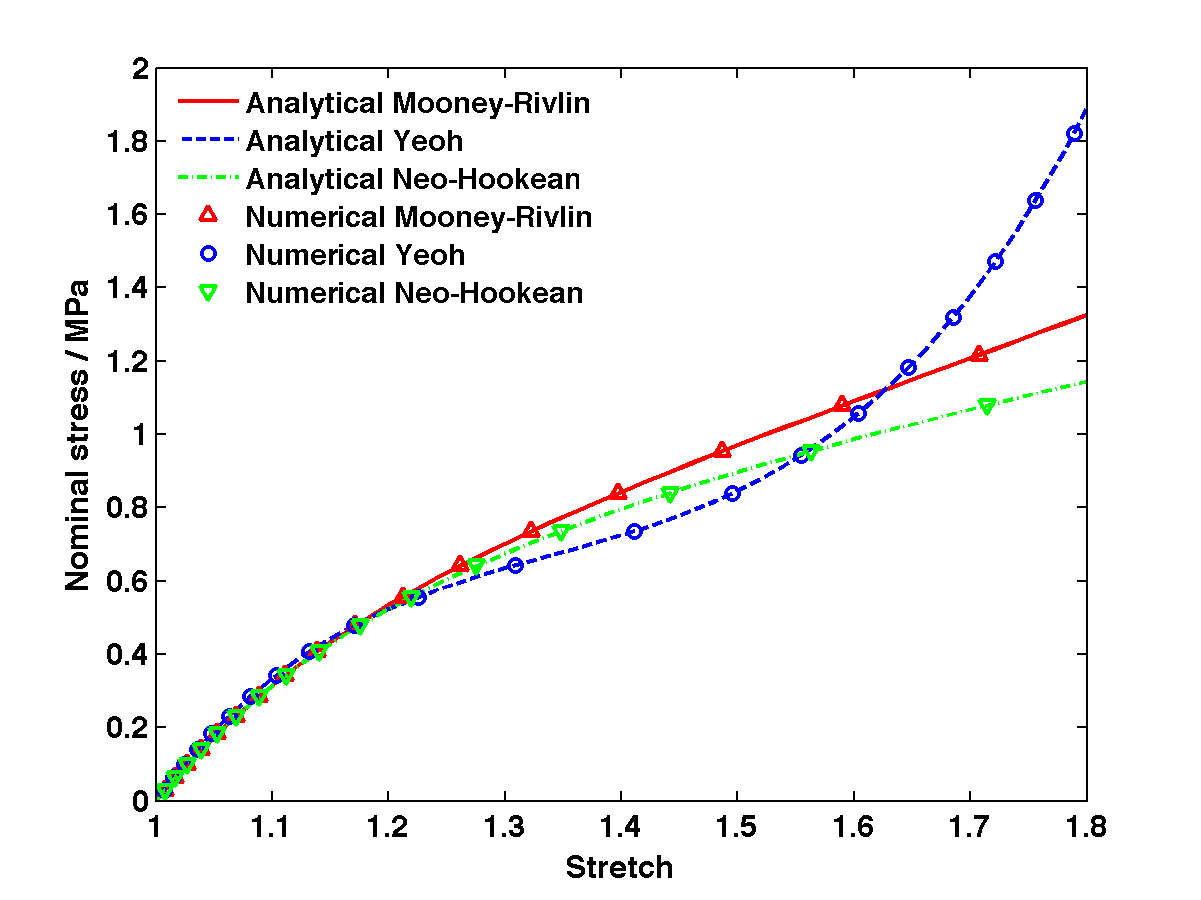
\includegraphics[width=.6\textwidth]{./figures/biaxial1.png}
\caption{Biaxial Tension Test for Isotropic Models}
\label{fig:biaxial1}
\end{figure}

To demonstrate the anisotropy of HGO model, we use the same material constant as the Neo-Hookean model before in the ground material. But only one direction is strengthened. That is, both two families of fibers are arranged in the $x$ direction. The material parameters in the anisotropic part are $k_1 = 10$ Pa and $k_2 = 20$ Pa. From Figure \ref{fig:biaxial2}, it is clear to see that stretch in $x$ direction is significantly less than $y$ direction. Along the non-strengthened $y$ direction, the stretch is approximately the same as Neo-Hookean model. While along the strengthened $x$ direction, the material is close to Neo-Hookean at first, then becomes very stiff. 
 
\begin{figure}[h!]
\centering
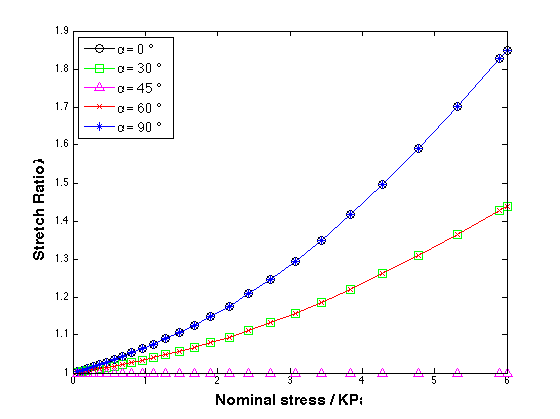
\includegraphics[width=.6\textwidth]{./figures/biaxial2.png}
\caption{Biaxial Tension Test for HGO Model}
\label{fig:biaxial2}
\end{figure}

\subsection{Cylindrical Pressure Vessel}